\section{Theorie}
\label{sec:Theorie}

Nur wenn $\beta$-Strahlung und $\gamma$-Strahlung auf Teilchen trifft, lässt sich eine Wechselwirkung feststellen.
Da innerhalb der Materie zwischen den Teilchen viel Freiraum ist, wird der Wirkungsquerschnitt $\sigma$ definiert.
Dieser gibt die Wahrscheinlichkeit innerhalb eines Raumanteils an, dass die Strahlung mit den Teilchen wechselwirkt.
Er steht somit in keinem direkten Verhältnis zu tatsächlichen geometrischen Größen.
Allerdings ist die Anzahl der Wechselwirkungen von der Dicke D des Absorbermaterials abhängig.
Dadurch ergibt sich für $\gamma$-Strahlung eine exponentieller Abfall.

\begin{equation}
  N(D) = N_0 \cdot \symup{e}^{-n \sigma D}
  \label{eqn:expo}
\end{equation}

N(D) bezeichnet hierbei die Anzahl der Teilchen, die nach dem Durchgang durch das Absorbermaterial noch vorhanden sind, n die Materieteilchen pro Volumeneinheit und $N_0$ die Anzahl der Teilchen pro Zeiteinheit, die auf die Fläche des Absorbers treffen.
Dies gilt auch für $\beta$-Strahlung bei geringen Dicken.
Es wird nun $n \cdot \sigma$ als der Absorptionskoeffizient $\mu$ definiert.
Die Materieteilchen pro Volumeneinheit können folgendermaßen berechnet werden:

\begin{equation}
  n = \frac{z N_A}{V_\text{Mol}}
  \label{eqn:n}
\end{equation}

Hierbei bezeichnet z die Ordnungszahl, $N_A$ die Avogrado-Konstante un V$_\text{Mol}$ das Molare Volumen.

\subsection{Absorption von \texorpdfstring{$\gamma$}{Gamma}-Strahlung}

Die Kerne eines Atom besitzen diskrete Energiezustände.
Wechseln die Kerne von einem energetisch höheren Zustand in einen energetisch niedrigeren so setzen sie Energie in Form von $\gamma$-Quanten frei.
Bei diesen $\gamma$-Quanten handelt es sich um Strahlung, die aus Photonen besteht.
Sie weist somit ebenso Teilchen-, wie auch Welleneigenschaften auf.
Bei der Wechselwirkung von $\gamma$-Strahlung mit Materie treten sehr viele Prozesse auf.
Die drei wichtigsten sind der innere Photo-Effekt, der Compton-Effekt und die Paarerzeugung.
Sie alle dominieren für verschiedene Energiebereiche der Strahlung, so dass sich eine sehr komplizierte Absorptionskurve ergibt.
Diese ist in Abbildung \ref{fig:Gammaabsorption} für Germanium dargestellt.

\begin{figure}
  \centering
  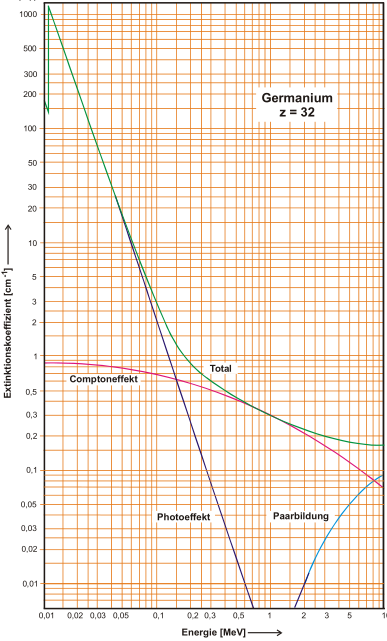
\includegraphics[scale=0.7]{pictures/Gammaabsorption.png}
  \caption{Die Energieabhängigkeit des Absorptionskoeffizienten für Germanium der verschiedenen Absorptionsprozesse, entnommen der Versuchsanleitung \cite[236]{sample}.}
  \label{fig:Gammaabsorption}
\end{figure}

Der Photoeffekt spielt für niedrige Energien von weniger als $\SI{200}{\kilo\electronvolt}$ eine große Rolle.
Hier tritt das Elektron in Wechselwirkung mit einem Hüllenelektron und wird vernichtet.
Die Energie wird dabei an das Elekton abgegeben, welches dadurch aus der Hülle asutritt.
Dies ist allerdings nur möglich, wenn die Energie der $\gamma$-Strahlung größer als die der Bindungsenergie ist.
Aus dem Impulssatz der Quantenmeschanik ergibt sich allerdings, dass der Atomkern einen Teil des Impulses aufnimmt.
Die Impulsübertragung ist hingegen nur für Elektronen wahrscheinlich, die fest an das Atom gebunden, also sehr nahe am Kern liegen.
Sie tritt somit für Elektronen der innersten Schale am häufigsten auf.
Dies erklärt auch, warum die Absorption von $\gamma$-Strahlung bei großen Atomen stärker auftritt.
Die Bindungsenergie der Elektronen in der K-Schale wächst ungefähr mit $Z^2$ an.
Die Übertragung des Impulses ist allerdings nur für geringe Energien wahrscheinlich, die Wahrscheinlichkeit der Absorption nimmt also für höhere Quantenenergien ab.


Der Compton-Effekt hingegen tritt bei der Streuung von $\gamma$-Strahlung an einem freien Elektron auf.
Es wird die Energie und die Richtung der $\gamma$-Strahlung verändert.
Auch hierbei wird Energie an das Elektron abgegeben, allerdings nicht die komplette.
nach erfolgter Wechselwirkung bleibt somit noch ein $\gamma$-Quant übrig.
Dessen Impuls zeigt in eine andere Richtung als die des Ursprungsquants.
Die $\gamma$-Strahlung wird somit aufgespalten und es kommt zu einer Intensitätsabnahme.
Nach Klein und Nishina kann der Wirkungsquerschnitt nach

\begin{equation}
  \sigma_{com} = 2 \pi r^2_e \left(\frac{1+\upvarepsilon}{\upvarepsilon^2} \left(\frac{2(1+\upvarepsilon)}{1+2\upvarepsilon} - \frac{1}{\upvarepsilon} \ln(1+\upvarepsilon)\right) + \frac{1}{2\upvarepsilon} \ln(1 + 2\upvarepsilon) - \frac{1+3\upvarepsilon}{(1+2\upvarepsilon)^2}\right)
  \label{eqn:sigmacom}
\end{equation}
berechnet werden.
Hierbei ist $r_e$ der klassische Elektronenradius mit $\SI{2.82e-15}{\metre}$ und $\upvarepsilon$ das Verhältnis der Energie der $\gamma$-Quanten zur Ruheenergie des Elektrons.
Die $\gamma$-Strahlung weist dabei eine mittlere Energie von über $\SI{200}{\kilo\electronvolt}$ und weniger als $\SI{1}{\mega\electronvolt}$ auf.


Bei großen Energien von über $\SI{1}{\mega\electronvolt}$ kann die sogenannte Paarerzeugung auftreten.
Hierbei wird das $\gamma$-Quant unter Bildung eines Elektrons und eines Positrons vernichtet.
Auch bei diesem Vorgang muss der quantenmechanische Impulssatz erfüllt sein.
Die Energie muss wieder von einem weiteren Partner, hier meist dem Atom, in dessen Coulomb-Feld sich das Elektron und Positron gebildet haben, übernommen werden.


Bei Durchtreten der $\gamma$-Strahlung durch ein Absorbermaterial überlagern sich alle oben genannten Effekte.
Die so entstehende Totalkurve ist relativ kompliziert und ist in Abbildung \ref{fig:Gammaabsorption} dargestellt.
\FloatBarrier
\subsection{Absorption von \texorpdfstring{$\beta$}{Beta}-Strahlung}
Die $\beta$-Strahlung ensteht durch die Umwandlung eines Neutrons in ein Proton, oder eines Protons in ein Neutron und besteht aus Elektronen beziehungsweise Positronen.
Zusätzlich entsteht noch ein Neutrino beziehungsweise Antineutrino.
Dies wird durch folgende Gleichungen beschrieben:
\begin{align*}
  p & \Rightarrow \: n \: + \: {\beta}^{+} \: + \: \nu_\text{e} \\
  n & \Rightarrow \: p \: + \: {\beta}^{-} \: + \: \overline{\nu_\text{e}}
\end{align*}
Die freiwerdende Energie verteilt sich statistisch auf die entstehenden Teilchen.
Das Spektrum eines $\beta$-Strahlers ist somit, wie in Abbildung \ref{fig:betaspektrum}
zu sehen, ein kontinuierliches.
\begin{figure}
  \centering
  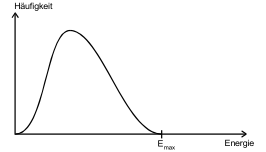
\includegraphics{pictures/betaspektrum.png}
  \caption{Emissionspektrum eines Beta-Strahlers.\cite{sample}}
  \label{fig:betaspektrum}
\end{figure}
Bei der Absoprtion von $\beta$-Strahlung am Festkörper treten eine Vielzahl von Prozessen auf.
Zum einen erleiden die Elek- und Positronen elastische Stoßprozesse. Dies führt zur Rutherfordstreuung.
Dabei werden die $\beta$-Teilchen durch Stöße mit den Atomen im Festkörper beziehungsweise deren Coulomb-Feld gestreut. Dabei kommt es zu keinen großen Energieverlust der Strahlung,
jedoch nimmt die Intensität der Strahlung durch die große Streuung stark ab.
Bei der inelastischen Streuung an den Atomkernen werden die geladenen $\beta$-Teilchen im Coulombfeld der Atome abgebremst und erzeugen sogenannte Bremsstrahlung.
Der Energieverlust durch die Bremsstrahlung ist jedoch für natürliche $\beta$-Strahler relativ gering.
Wesentlich höher ist der Energieverlust durch inelastische Stöße mit den Elektronen des Festkörpers. Dabei treten Ionisations- und Anregungsprozesse an den Atomen auf.
Bei diesen Prozessen verliert das $\beta$-Teilchen zwar nur eine geringe Energiemenge, jedoch treten, vorallem bei Metallen, viele dieser Prozesse hintereinader auf und
bremsen die Strahlung stark ab. Da eine einheitliche analytische Beschreibung unter Berücksichtigung all dieser Absorptionsprozesse sehr schwierig ist, wird im Folgenden
mit empirisch ermittelten Gesetzmäßigkeiten gearbeitet. So zeigt sich grafisch der in Abbildung \ref{fig:betaabsorption} zu sehende Zusammenhang zwischen durchgehender Intensität
und der Massenbelegung $R=\rho D$.

\begin{figure}
  \centering
  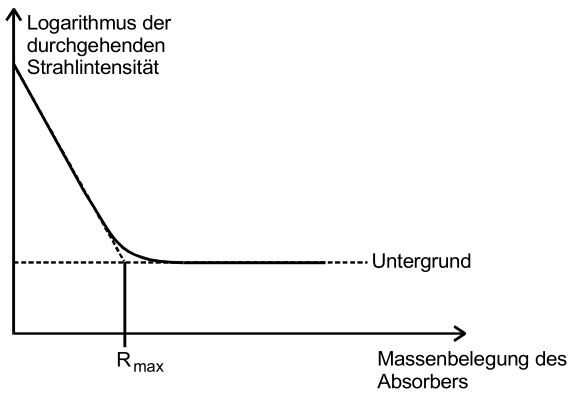
\includegraphics[scale=0.7]{pictures/betaabsorption.png}
  \caption{Schematische Darstellung der Absorptionskurve eines Beta-Strahlers.\cite{sample}}
  \label{fig:betaabsorption}
\end{figure}

Aus dem aus der Grafik \ref{fig:betaabsorption} ermittelten $R_\text{max}$ lässt sich nun die maximale Energie der $\beta$-Strahlung mit

\begin{equation}
  E_\text{max} = 1,92 \sqrt{{R_\text{max}}^2 + 0,22 R_\text{max}} \cdot [\si{\mega\electronvolt}]
  \label{eqn:betaenergie}
\end{equation}

berechnen. $R_\text{max}$ ist dabei in $\si{\gram\per\centi\metre\squared}$ einzusetzen.

\FloatBarrier
